\documentclass[addpoints,spanish, 12pt,a4paper]{exam}
\pointpoints{punto}{puntos}
\hpword{Puntos:}
\vpword{Puntos:}
\htword{Total}
\vtword{Total}
\hsword{Resultado:}
\hqword{Ejercicio:}
\vqword{Ejercicio:}
\usepackage{pgf,tikz}
\usetikzlibrary{shapes, calc, shapes, arrows, math, babel}

% \printanswers

\usepackage[utf8]{inputenc}
\usepackage[spanish]{babel}
\usepackage{eurosym}
\usepackage{yhmath}
%\usepackage[spanish,es-lcroman, es-tabla, es-noshorthands]{babel}

\usepackage{verbatim}

\usepackage[margin=1in]{geometry}
\usepackage{amsmath,amssymb}
\usepackage{multicol}

\usepackage{graphicx}
\graphicspath{{../img/}} 

\newcommand{\class}{Matemáticas 4º Aplicadas}
\newcommand{\examdate}{\today}
\newcommand{\examnum}{Funciones y Estadística}
\newcommand{\tipo}{A}


\newcommand{\timelimit}{50 minutos}

\renewcommand{\solutiontitle}{\noindent\textbf{Solución:}\enspace}

\pagestyle{head}
\firstpageheader{
\includegraphics[width=0.2\columnwidth]{header_left}}{\textbf{Departamento de Matemáticas\linebreak \class}\linebreak \examnum}{
\includegraphics[width=0.1\columnwidth]{header_right}}
\runningheader{\class}{\examnum}{Página \thepage\ of \numpages}
\runningheadrule

\pointsinrightmargin % Para poner las puntuaciones a la derecha. Se puede cambiar. Si se comenta, sale a la izquierda.
\extrawidth{-2.4cm} %Un poquito más de margen por si ponemos textos largos.
\marginpointname{ \emph{\points}}


\begin{document}

\noindent
\begin{tabular*}{\textwidth}{l @{\extracolsep{\fill}} r @{\extracolsep{6pt}} }
\textbf{Nombre:} \makebox[3.5in]{\hrulefill} & \textbf{Fecha:}\makebox[1in]{\hrulefill} \\
 & \\
\textbf{Tiempo: \timelimit} & Tipo: \tipo 
\end{tabular*}
\rule[2ex]{\textwidth}{2pt}
Esta prueba tiene \numquestions\ ejercicios. La puntuación máxima es de \numpoints. 
La nota final de la prueba será la parte proporcional de la puntuación obtenida sobre la puntuación máxima. 

% Para la evaluación de pendientes de 3ºESO o 2ºPMAR se tendrán en cuenta los apartados 1.a, 1.c, 1.d, 2.a y 4:
\begin{center}


\addpoints
 %\gradetable[h][questions]
	\pointtable[h][questions]
\end{center}

\noindent
% \textbf{NOTA:} Los problemas se han de resolver mediante ecuaciones o sistemas. Y los ejercicios mediante métodos diferentes a la resolución por tanteo.
% \rule[2ex]{\textwidth}{2pt}

\begin{questions}

\question La gráfica representa un viaje en coche, obsérvala y responde a las preguntas:

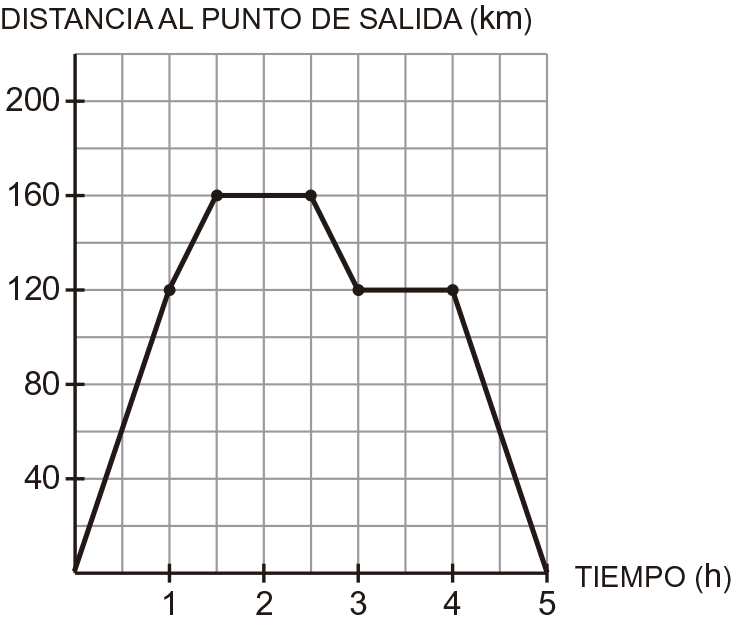
\includegraphics[]{viaje}

\begin{parts}

\part[1] ¿Cuántos kilómetros recorre en la primera hora?
 
\part[1] ¿Cuánto tiempo permanece parado?
 
\part[1] ¿A qué distancia del punto de partida se encuentra el lugar de la segunda parada?
 
\part[1] ¿Cuánto tiempo duró el viaje en total?
 
\part[1] ¿Cuáles son las variables dependiente e independiente? 

\end{parts}

% \question Las siguientes gráficas muestran la media de las temperaturas máximas alcanzadas en Varsovia y en Praga durante el año pasado:

% 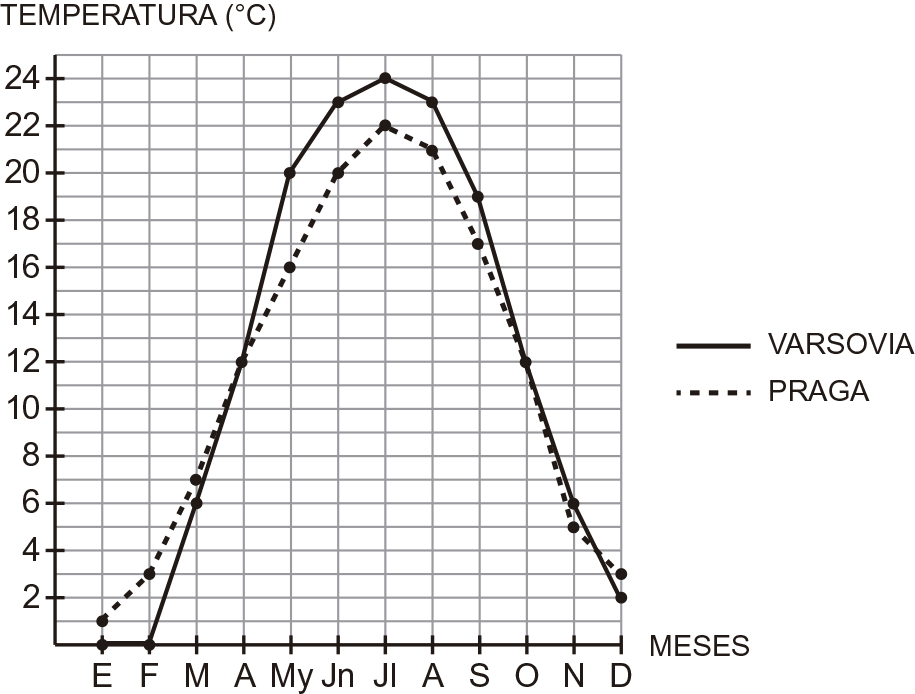
\includegraphics[]{temperaturas}
% \begin{parts}
% \part[2] ¿Entre qué mes alcanza la mayor temperatura Praga y Varsovia?
% \part[2] ¿Cuál de las dos capitales es la más fría en invierno?
% \part[2] ¿En qué mes se produce la mayor diferencia de temperatura entre ambas ciudades?
% \part[2] ¿En qué ciudad es mayor la diferencia entre la temperatura máxima y la mínima?
% \end{parts}

\question A continuación se recogen las puntuaciones obtenidas al lanzar 50 veces un dado:
\begin{center}
1 3 4 2 1 3 4 5 6 3

4 3 5 4 6 4 3 2 5 4

6 3 2 4 1 2 2 4 5 5

6 3 5 2 5 4 3 3 5 6

6 5 2 5 6 3 2 1 4 2
\end{center}
\begin{parts}
\part[1] Haz, con los resultados, una tabla con las frecuencias absolutas,
\part[1] Dibuja un diagrama de barras que refleje la información del apartado anterior
\part[1] Amplia la tabla anterior con las frecuencias relativas y el porcentaje correspondiente
\end{parts}


\question Se preguntó a cierto grupo de 25 estudiantes de Bachillerato las veces que fueron al cine durante el año pasado. Sus respuestas se recogen en la siguiente tabla. Calcula la media, la moda y la desviación media.
\begin{center}
\begin{tabular}{|c |c |}\hline
Nº veces & Frecuencia \\ 
\hline
$4$&$4$\\
\hline
$5$&$3$\\
\hline
$6$&$6$\\
\hline
$7$&$7$\\
\hline
$8$&$5$\\
\hline
\end{tabular}
\end{center}

\begin{parts}
\part[1] Calcula la media
\begin{solution}
\end{solution}
\part[1] Calcula la moda
\begin{solution}
\end{solution}
\part[1] Calcula la mediana
\begin{solution}
\end{solution}
\part[1] Calcula la desviación media
\begin{solution}
\end{solution}

\end{parts}



\question Una compañía de teléfonos me cobra una cantidad fija al mes: 1 \euro . Además me cobran 50 céntimos por cada hora de llamadas. Queremos reflejar en forma de función la factura mensual (lo que pago al mes)
\begin{parts}
% \part[1] ¿Cuáles son la variables dependientes e independientes de la función?
% \begin{solution}
% $x$ = tiempo, $y$ = dinero
% \end{solution}
\part[1] Haz una tabla de valores que refleje dicha variable

\begin{solution}
\begin{center}
\begin{tabular}{|c |c |}\hline
$x$ & $y$\\ 
\hline
$1$&$1.5$\\
\hline
$2$&$2$\\
\hline
$3$&$2.5$\\
\hline
$4$&$3$\\
\hline
\end{tabular}
\end{center}
\end{solution}
\part[1] Representa gráficamente los valores anteriores y únelos para determinar la gráfica de la función\\
\begin{tikzpicture}[line cap=round,line join=round,>=triangle 45,x=1cm,y=1cm, scale=0.4]
\draw [color=lightgray,dash pattern=on 1pt off 1pt, xstep=1cm,ystep=1cm] (-3.6,-3.4) grid (20.1,10.1);
\draw[<->,color=black] (-3.6,0) -- (20.1,0);
\foreach \x in {-3,-2,-1,1,2,3,4,5,6,7,8,9,10,11,12,13,14,15,16,17,18,19,20}
\draw[shift={(\x,0)},color=black] (0pt,1pt) -- (0pt,-1pt) node[below] {\footnotesize $\x$};
\draw[<->,color=black] (0,-3.43158220601634095) -- (0,10.1);
\foreach \y in {-3,-2,-1,1,2,3,4,5,6,7,8,9,10}
\draw[shift={(0,\y)},color=black] (2pt,0pt) -- (-2pt,0pt) node[left] {\footnotesize $\y$};
%\draw[color=black] (0pt,-10pt) node[right] {\footnotesize $0$};
%\clip(-0.6129302567150502,-0.43158220601634095) rectangle (9.010648940148005,7.8783927087822985);
\end{tikzpicture}
\begin{solution}
\begin{tikzpicture}[line cap=round,line join=round,>=triangle 45,x=1cm,y=1cm, scale=0.4]
\draw [color=lightgray,dash pattern=on 1pt off 1pt, xstep=1cm,ystep=1cm] (-3.6,-3.4) grid (20.1,10.1);
\draw[<->,color=black] (-3.6,0) -- (20.1,0);
\foreach \x in {-3,-2,-1,1,2,3,4,5,6,7,8,9,10,11,12,13,14,15,16,17,18,19,20}
\draw[shift={(\x,0)},color=black] (0pt,1pt) -- (0pt,-1pt) node[below] {\footnotesize $\x$};
\draw[<->,color=black] (0,-3.43158220601634095) -- (0,10.1);
\foreach \y in {-3,-2,-1,1,2,3,4,5,6,7,8,9,10}
\draw[shift={(0,\y)},color=black] (2pt,0pt) -- (-2pt,0pt) node[left] {\footnotesize $\y$};
%\draw[color=black] (0pt,-10pt) node[right] {\footnotesize $0$};
%\clip(-0.6129302567150502,-0.43158220601634095) rectangle (9.010648940148005,7.8783927087822985);
\draw[->, color=red, domain=0  :16 + 0.1]    plot (\x,{1/2*(\x) + 1}) node[right] {};
\end{tikzpicture}

\end{solution}
\part[2] Da la expresión analítica (o algebraica) de la función
\begin{solution} $y=0.5x+1$
\end{solution}
\part[2] A partir de la expresión analítica, calcula cuánto me facturarán si un mes hablo 200 horas
\begin{solution}
$y=0.5\cdot200+1=101$\euro
\end{solution} 
% \part[1] Determina el dominio y el recorrido de la función
\end{parts}





\addpoints

\end{questions}

\end{document}
